% TODO: Remove
\addbibresource{../report.bib}

\section{Attack Design and Implementation}

In this section, we describe the design of our automatic feature generation model, outline the attack strategy and explain certain design decisions.
Most of this section will be split into two different sections.
First we describe the feature generation process and then the overall attack.

\subsection{Sequence-to-Sequence Model}

As described in section \ref{sec:seq2seq}, a sequence-to-sequence model is able to learn how to construct a fixed-length representation from a variable-length sequence.
However, here we outline the exact structure of the model and show the implementation in Tensorflow.

\subsubsection{Overall Structure}

One of the parameters, which has a large impact on the accuracy of the reconstruction process is the \textit{amount of hidden states} in the RNN cells.
Every neural network layers within a cell has a given amount of neurons.
Hence, if for example the amount of hidden neurons is set to $100$, our state at every cell is represented by vector of length $200$ (since the state is represented by two vectors of length $100$).
The higher this number, the easier it should be to learn a representation, as the compression factor is lower.
But we also need to consider the fact that the higher the amount of hidden neurons, the more variables the model needs to learn.

Each value in a trace can be represented by a vector of length two (timestamp and direction), as seen in table \ref{table:cell-extract}.
Therefore, if the amount of hidden cells is not equal to two, we will also need to \textit{project} the input and output to the necessary dimensions.

\begin{figure}[ht]
  \centering
  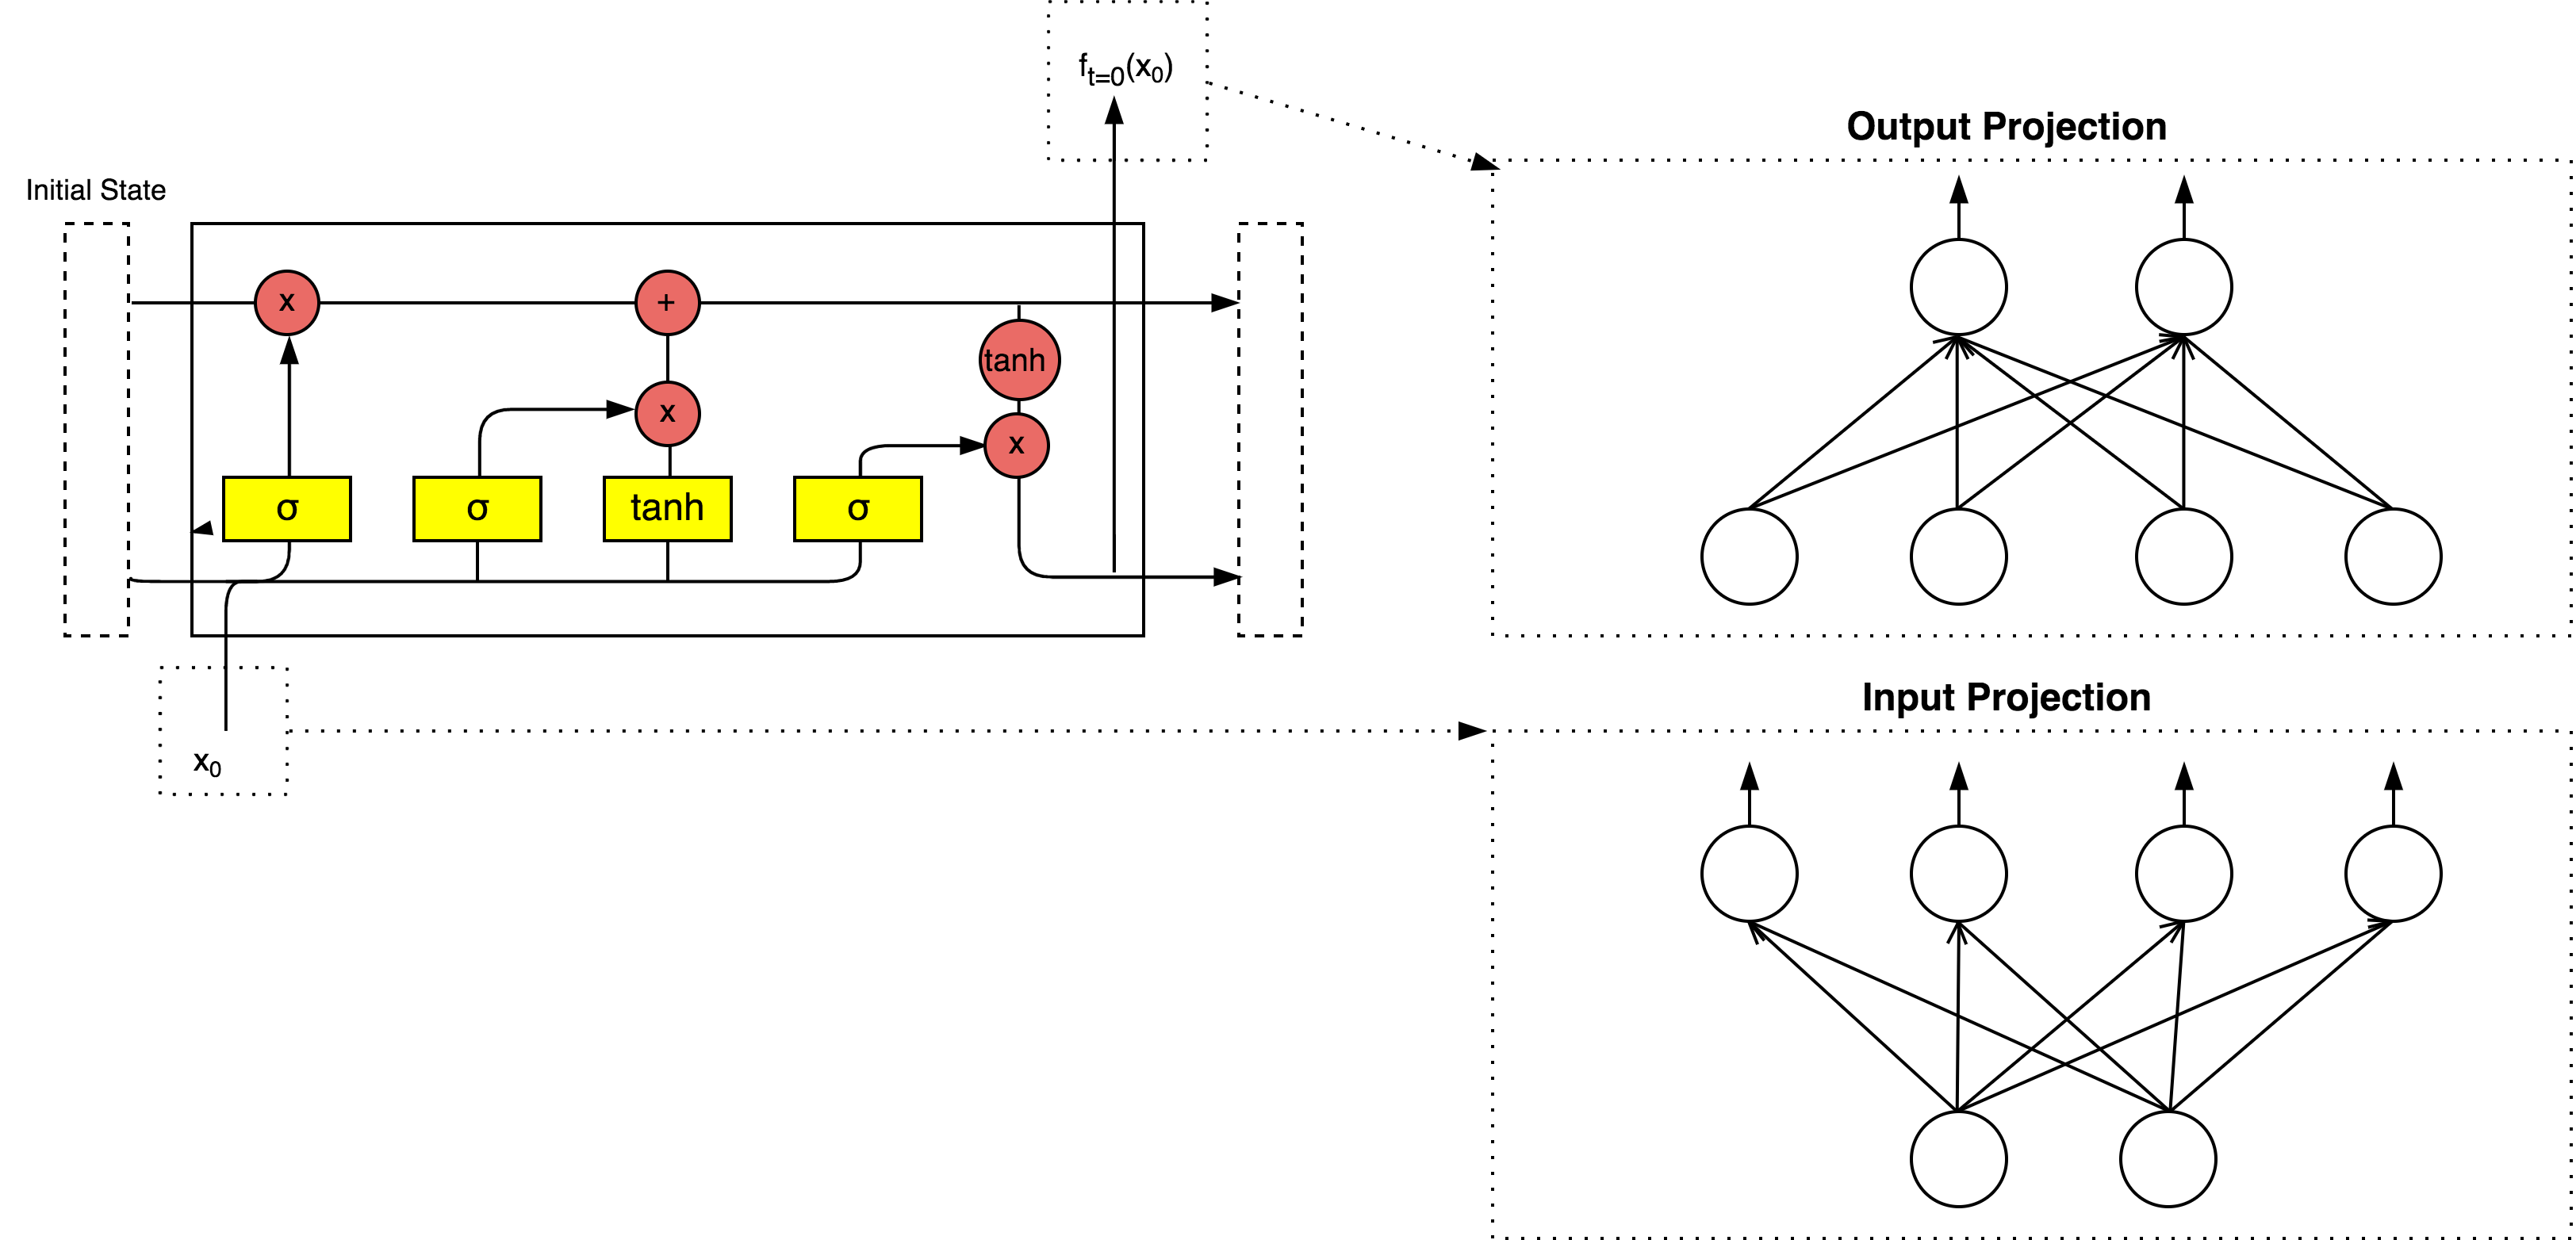
\includegraphics[width=0.7\textwidth]{lstm-projection}
  \caption{Example of projection within a LSTM cell with 4 hidden states.}
  \label{fig:lstm-projection}
\end{figure}

Some of the traces can be particularly long and therefore the network needs to be unrolled to extreme lengths \cite{greschbach2016effect}.
In fact, given memory constraints, this issue can become a major problem.
This can be solved by cutting the traces after a couple seconds since it has been shown that the first part of a trace carries more information than the latter \cite{TODO: Include}.

\begin{figure}[ht]
  \centering
  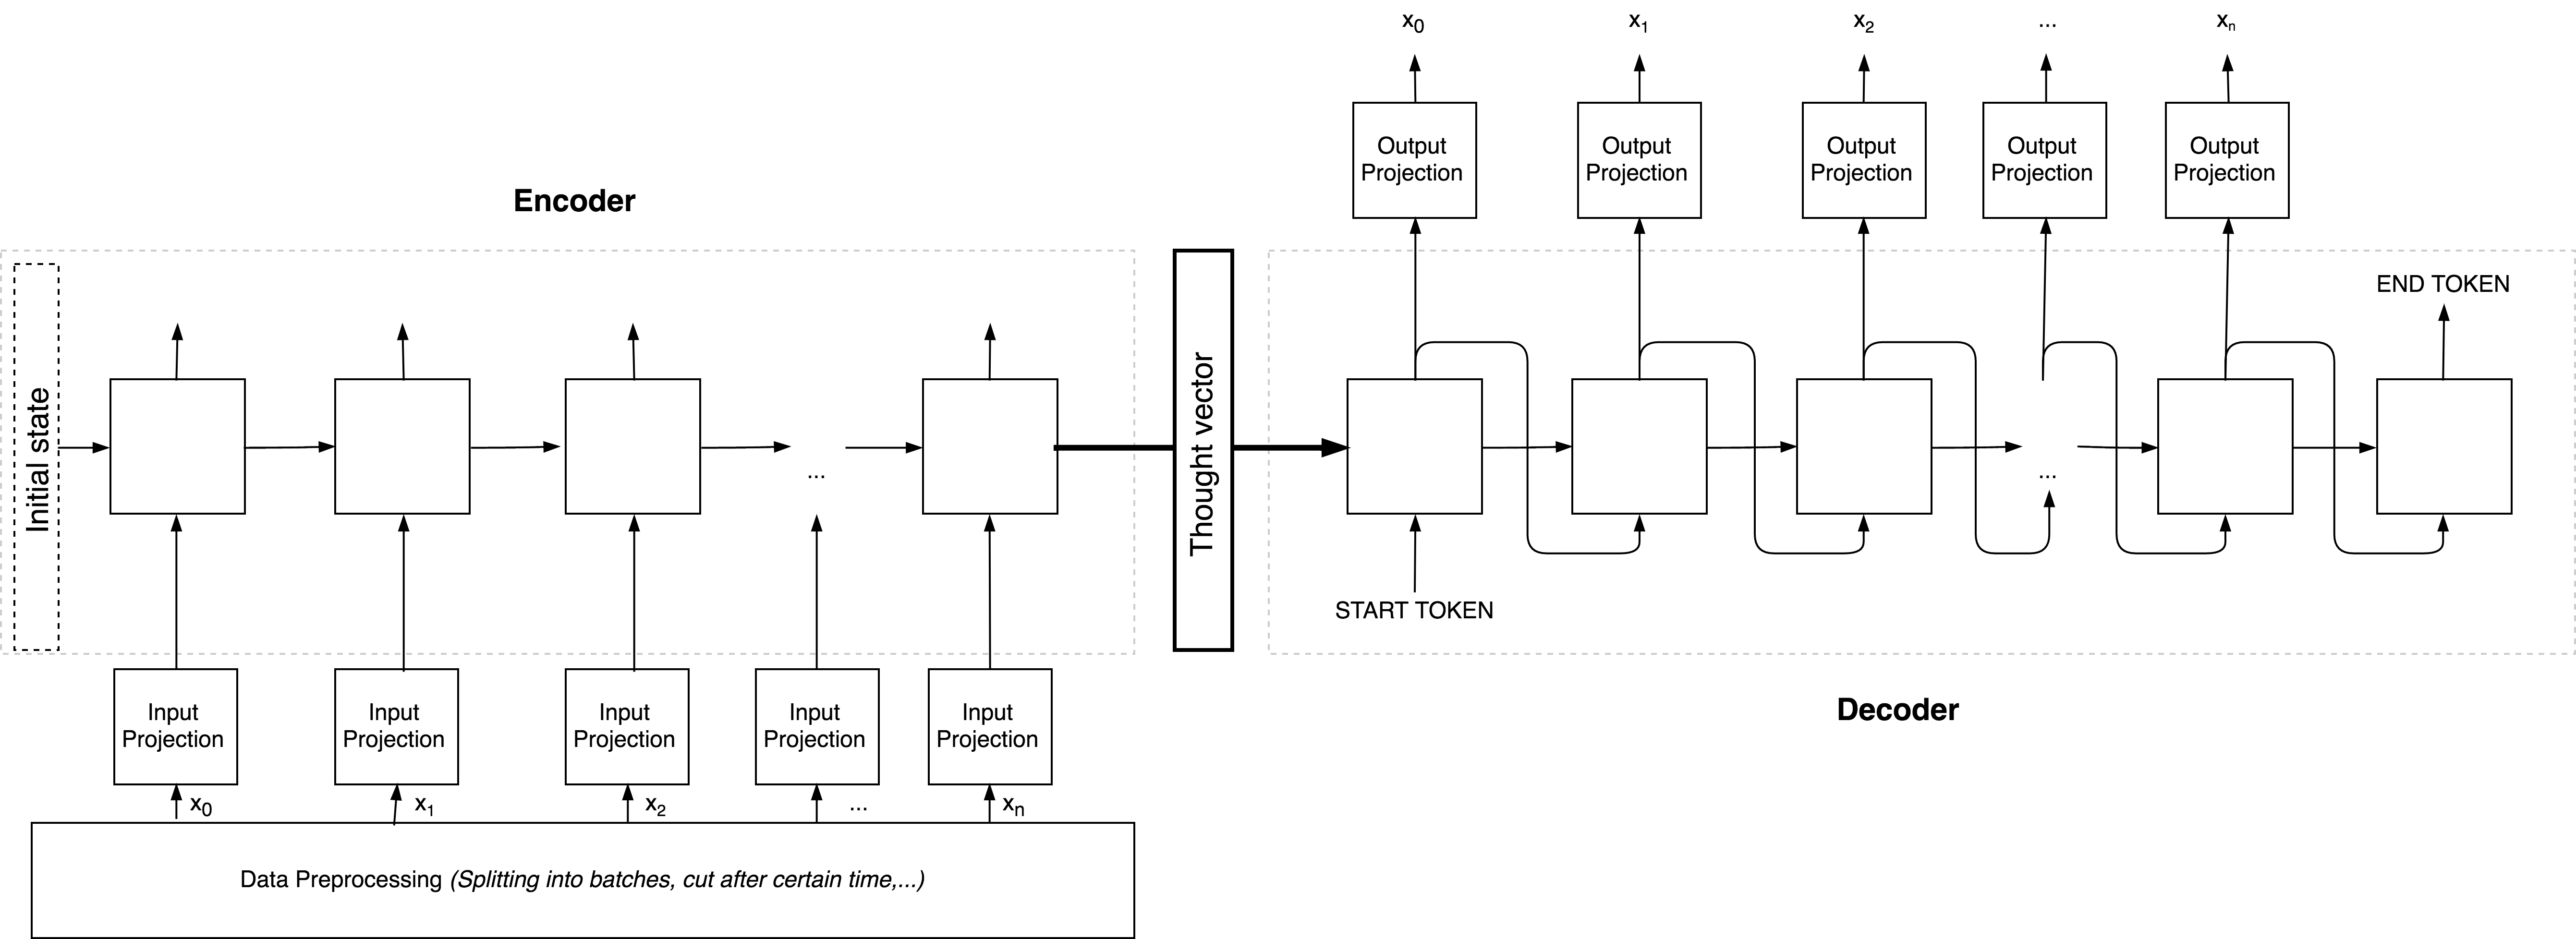
\includegraphics[width=\textwidth]{full-seq2seq}
  \caption{Overal structure of our sequence-to-sequence model.}
  \label{fig:full-seq2seq}
\end{figure}

\subsubsection{Implementation}

\subsection{Attack Strategy}

- Collect data on web pages you need to monitor
- Train deep learning model
- Extract features
- Train other model
- Capture traffic
- Classify new instances

% Figure of how design looks
% Description of each component
% Can I use deep learning to classify



% TODO: Where code is
